\chapter{System Proposal}
\label{cha:systemProposal}
%\noindent Descrição da arquitetura
%\begin{itemize}
%    \item Como recebemos dados dos IMU
%    \item Quando recebemos dados dos IMU (freq.)
%    \item 3 "Módulos" - Explicar cada um deles
%    \begin{enumerate}
%        \item Edge: sensores e raspberry Pi
%        \item Server
%        \item Client
%    \end{enumerate}
%    \item Comunicação entre os módulos
%\end{itemize}
%---------

\noindent To achieve the goals set in Chapter \ref{cha:introduction}, a system that collects and processes the raw data from the IMU sensors and transforms it into meaningful metrics, storing it, and then presents it in a clear way to the user has to be built.

The proposed architecture is shown in Figure~\ref{fig:architecure}, and it is comprised of three segments:

\begin{enumerate}
    \item \label{enum:segEdge} Edge - Data Collection and Processing
    \item \label{enum:segServer} Server - Data Storing and Application Server
    \item \label{enum:segClient} Client - Frontend Application
\end{enumerate}

\begin{figure}
    \centering
    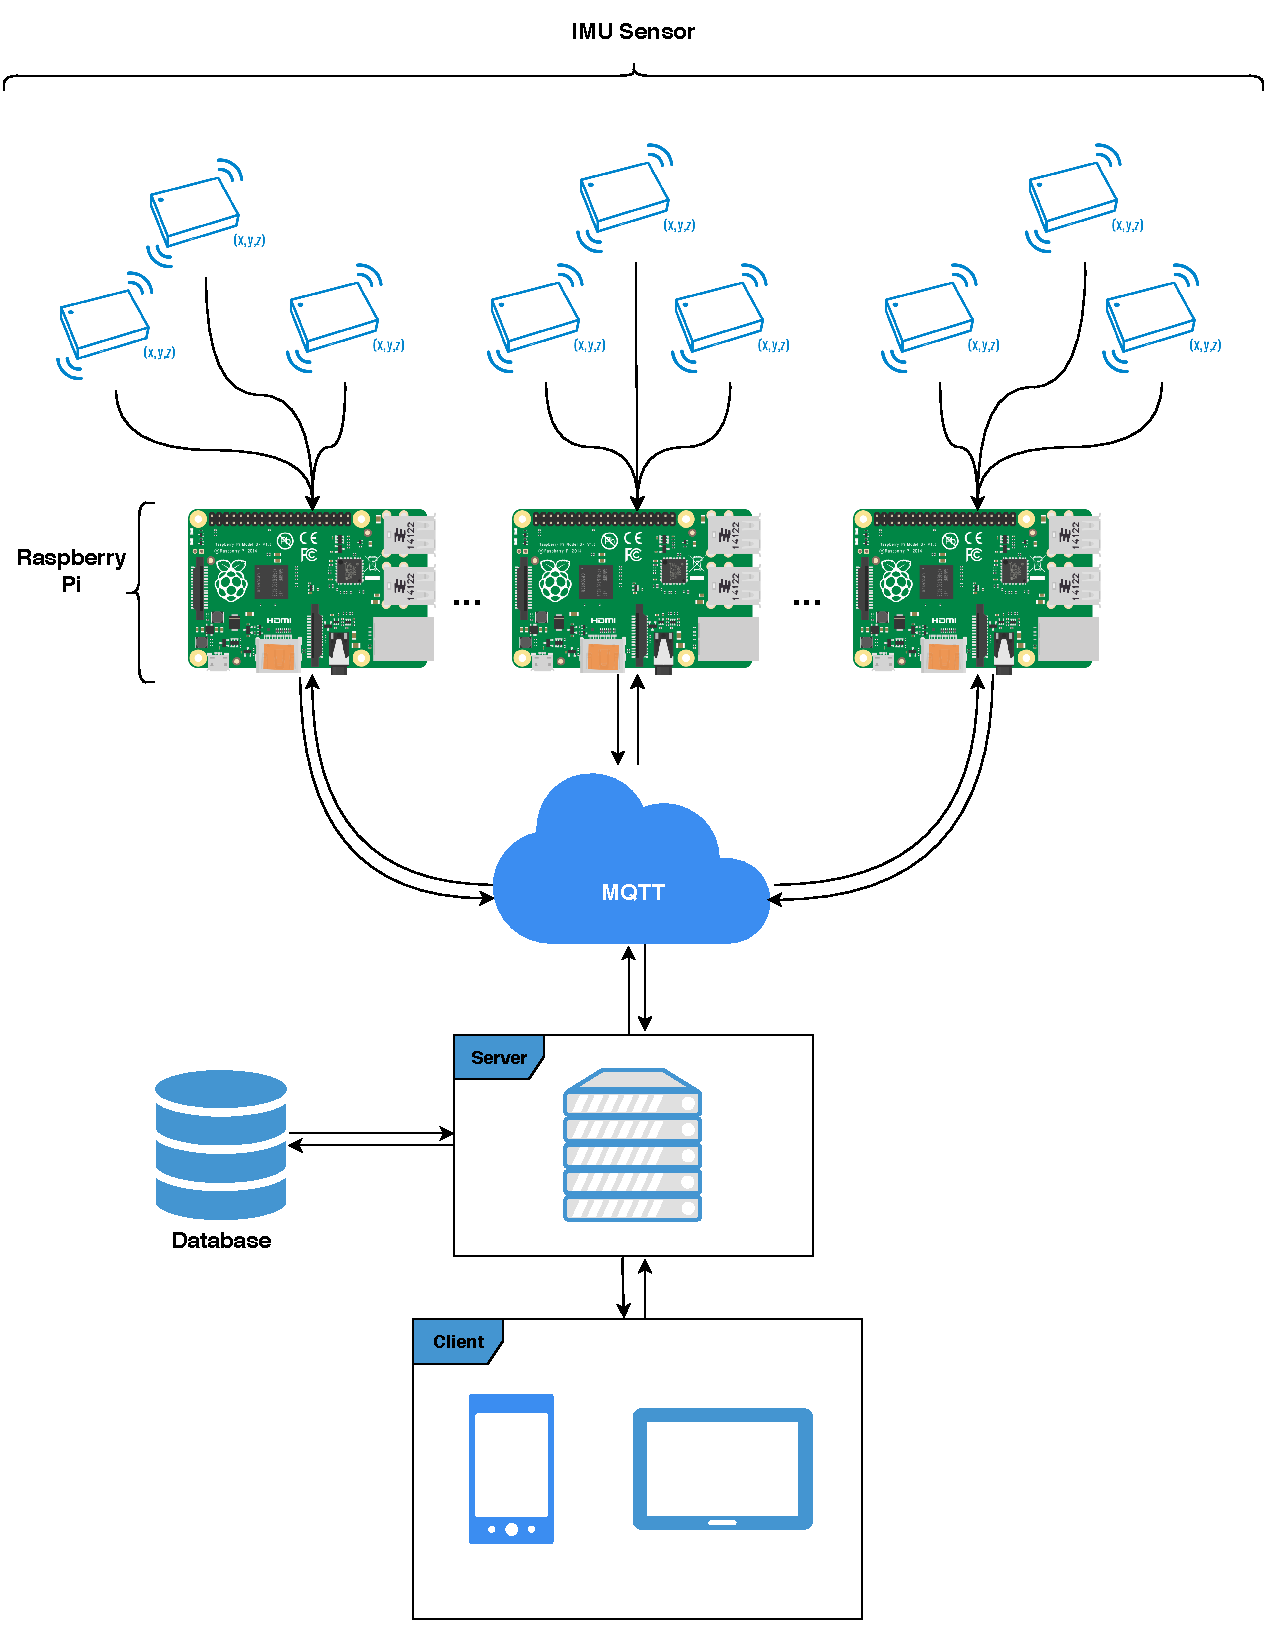
\includegraphics[width=.47\textwidth]{BLESportsTrackerArchitecture.pdf}
    \caption{Proposed Architecture}
    \label{fig:architecure}
\end{figure}

\section{Edge}
\label{sec:edge}
\noindent The Edge segment is composed of at least one IMU Sensor and one Raspberry Pi, connected via Bluetooth.

As the number of sensors can grow, and due to the limitation of the number of connections to a Bluetooth receiver, %http://dev.ti.com/tirex/content/simplelink_academy_cc26x2sdk_1_15_03_10/modules/ble5stack/ble_connections/ble_connections.html
the number of Raspberry Pi's can also grow, in order to establish connection with all the IMU Sensors. This also helps to share the computation of the game metrics between the Raspberry Pi's.

\subsection{IMU Sensors}
\label{subsec:imu}
\noindent The IMU sensors are attached to the players, and their only job is to send accelerometer and gyroscope raw data to the Raspberry Pi they are connected, over Bluetooth.

\subsection{Raspberry Pi}
\label{subsec:raspi}
\noindent In the Raspberry Pi is where the "hard" work is done. Besides connecting and controlling the IMU Sensors, this unit has two main jobs: to collect the raw data sent by the IMU Sensors several times per second, and perform calculations with the gathered data to measure in-game metrics, which are then broadcasted to the server, to be stored and shown to the User.


\section{Server}
\label{sec:server}
\noindent The Server is the main piece of the architecture, allowing the interaction between the User and the IMU Sensors.

The Server can broadcast instructions to the Raspberry Pi, controlling the IMU Sensors.
When data is received from the Raspberry Pi's, the Server stores it, so that it can be shown to the User.

The Server also hosts the Client Application, where it receives the instructions to be sent to the Edge, and it shows the received data to the User.

\section{Client}
\label{sec:client}
\noindent The Client Application provides the User an interface in which he can control the IMU Sensors, and displays the edge-computed in-game metrics.